
\section{Logic}
\subsection{Propositional logic}

\begin{definition*}
  An atom is a logical proposition which cannot be decomposed. A formula is a tree in which each
  node is either
  \begin{enumerate}
  \item an atom, or
  \item a logical operator with one child node for each argument.
  \end{enumerate}
  The logical operators are:
  \begin{itemize}
  \item $\lnot p$ negation
  \item $p \lor q$ disjunction
  \item $p \land q$ conjunction
  \item $p \limplies q$ implication
  \item $p \lequiv q$ equivalence
  \end{itemize}
  An interpretation is an assignment of true/false values to the atoms in a formula (well, except
  for logical constants, those are atoms but are constant true or constant false).

  A truth table is a list of all interpretations together with the resulting values of the formula.

  A model for a formula is an interpretation (row of truth table) for which the formula evaluates
  to true.

  A formula is satisfiable if there exists a model for it.

  A formula is valid (aka a tautology) if every interpretation is a model.

  The negation of a valid formula is not satisfiable.
\end{definition*}


\begin{theorem*}
  All other logical
\end{theorem*}

\newpage
\section{Combinatorics}

\begin{mdframed}
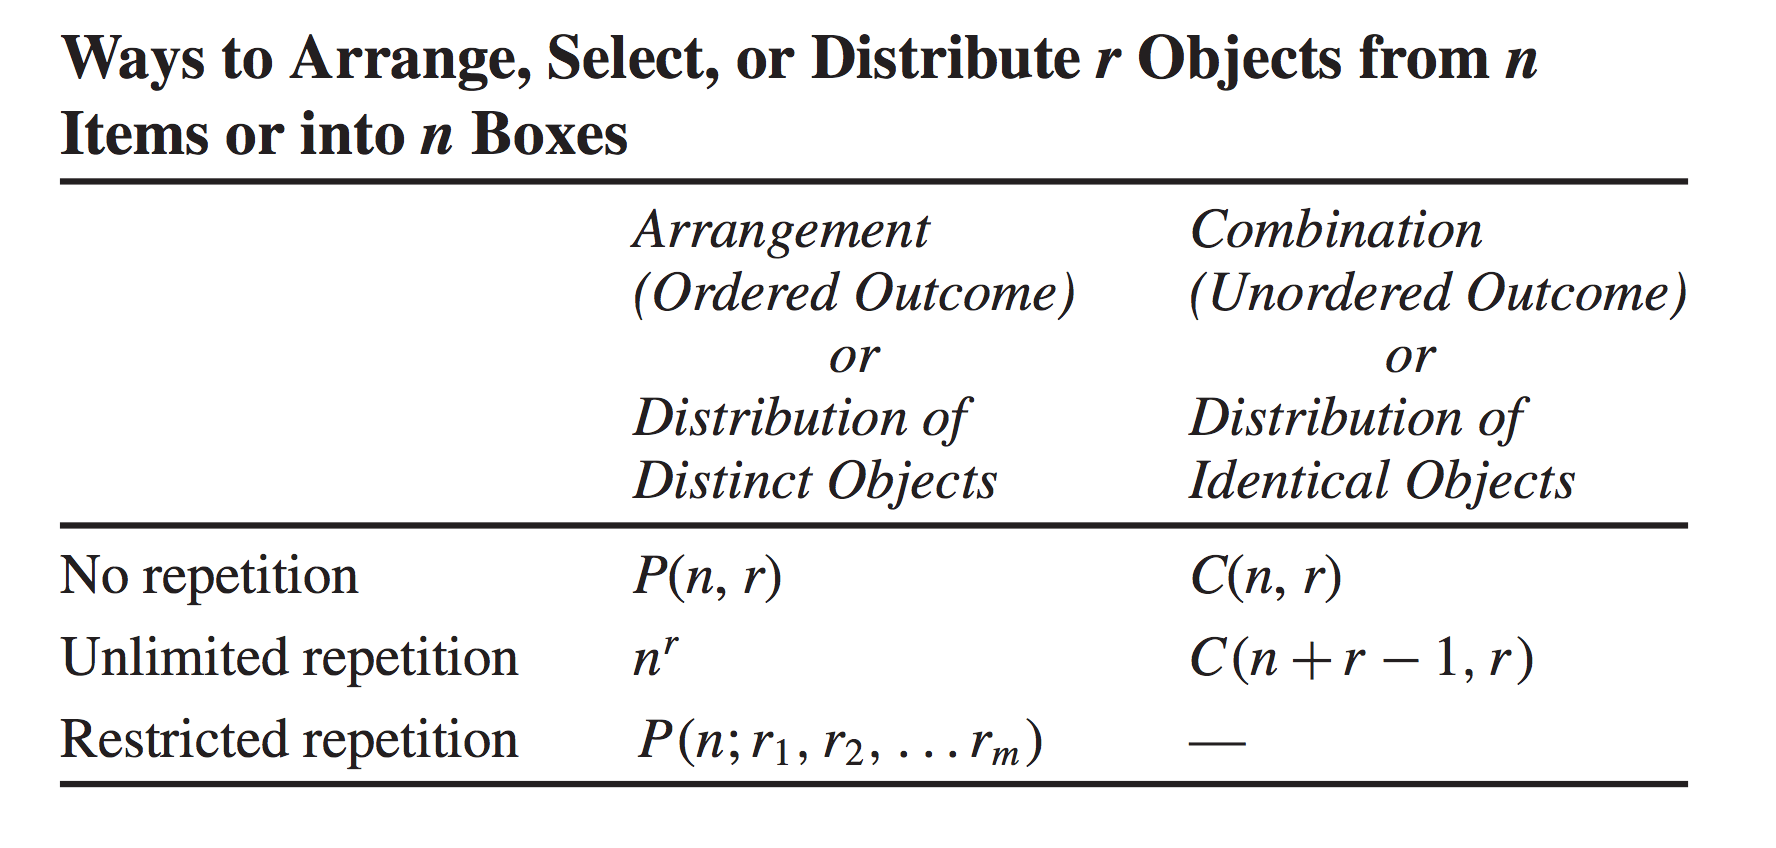
\includegraphics[width=300pt]{img/discrete-mathematics-tucker-combinatorics-summary.png}
\end{mdframed}

\begin{theorem*}[Subtuples]~\\
  The number of $k$-tuples that can be formed from a set of size $n$ without replacement is
  \begin{align*}
    (n)_k := n \cdot (n-1) \cdots (n - k + 1) = \frac{n!}{(n-k)!}.
  \end{align*}
\end{theorem*}

\begin{remark*}
  As a special case, the number of $n$-tuples (i.e. permutations/arrangements) is $n!$. (This is also
  the number of $n-1$ tuples.)
\end{remark*}

\begin{theorem*}[Subsets]~\\
  The number of subsets of size $k$ that can be formed from a set of size $n$ is
  \begin{align*}
    C(n, k) = {n \choose k} := \frac{(n)_k}{k!} = \frac{n!}{(n-k)!~k!}.
  \end{align*}
\end{theorem*}

\begin{proof}
  Each distinct $k$-subset gives rise to $k!$ $k$-tuples by assigning position labels. Therefore
  $(n)_k = {n \choose k}k!$.
\end{proof}

\begin{theorem*}[Multiset arrangements]~\\
  Consider a multiset comprising $n$ distinct elements, with $r_i \geq 1$ repeats of the $i$-th
  element. The number of $n$-tuples that can be formed from such a multiset is
  \begin{align*}
    P(n; r_1, \ldots, r_k)
    :=& {n \choose r_1}{n - r_1 \choose r_2}\cdots{n - r_1 \cdots - r_{n-1} \choose r_n}\\
    % &=\frac{n!}{(n - r_1)!r_1!}
    %   \frac{(n - r_1)!}{(n - r_1 - r_2)!r_2!}
    %   \cdots
    %   \frac{(n - r_1 \cdots - r_{n-1})!}{r_n!}
     =& \frac{n!}{r_1!r_2!\cdots r_n!}.
  \end{align*}
\end{theorem*}

\begin{proof}
  The $r_1$ copies of the first element must all go somewhere. ${n \choose r_1}$ counts the number
  of distinct positions they can occupy. Then there are $n - r_1$ empty positions left. Etc.
\end{proof}

\begin{remark*}
  The number $n!$ of permutations of a set is a special case of this with $r_i = 1$ for all $i$.
\end{remark*}

\begin{example*}~\\
  \begin{enumerate}
  \item {\bf How many ways are there to assign 100 different diplomats to five different
      continents?}\\
    $5^{100}$
  \item {\bf How many ways if 20 diplomats must be assigned to each continent?}\\
    $P(100; 20, 20, 20, 20, 20)$. Arrange the 100 diplomats in an arbitrary order. Now we have a
    multiset of country labels with 20 repeats of each label. Given the fixed ordering of the
    diplomats, there's a one-to-one correspondence between distinct permutations of the multiset
    and assignments of diplomats to countries.
  \item {\bf How many ways are there to distribute 20 (identical) sticks of red licorice and 15
    (identical) sticks of black licorice among five children?}\\
  ${20 + 5 -1 \choose 5 - 1}$${15 + 5 -1 \choose 5 - 1}$.
  \end{enumerate}
\end{example*}

\begin{theorem*}
  How many $k$-tuples for $k \leq n$ can be formed from such a multiset?
\end{theorem*}
\red{TODO}

\begin{theorem*}[Stars and bars]~\\
  Consider the number of ways that $n$ identical objects can be put into $k$ buckets, recording
  only the counts in each bucket (not the identities of the objects).

  With no empty buckets, the answer is
  \begin{align*}
    {n - 1 \choose k - 1} ~~~~~~~\text{($k-1$ bars to be placed in $n-1$ gaps between $n$ stars)}.
  \end{align*}

  With empty buckets allowed, the answer is
  \begin{align*}
    {n + k - 1 \choose k - 1} = P(n + k - 1; n, k - 1)~~~~~~~\text{(number of arrangements of $n$ stars and $k-1$ bars)}.
  \end{align*}
\end{theorem*}

\begin{proof}
  Represent this as $n$ unlabeled stars, and $k-1$ bars representing the partition of the stars
  into different buckets.

  With no empty buckets allowed, there are $n-1$ gaps where the bars can be placed, hence
  ${n - 1 \choose k - 1}$ ways of dividing up the items.

  With empty buckets allowed, there could be multiple bars in the same position. The number of
  $(n + k - 1)$-tuples that can be formed from the star and bar symbols is
  \begin{align*}
    P(n + k - 1; n, k - 1) &= C(n + k - 1, k - 1)C(n, n)\\
                           &= C(n + k - 1, k - 1)\\
                           &= C(n + k - 1, n)C(k - 1, k - 1)\\
                           &= C(n + k - 1, n).
  \end{align*}

  Note that ${n - 1 \choose k - 1}$ for the no-empty-buckets version can also be derived as
  follows:
  \begin{enumerate}
  \item Place one item into each bucket.
  \item Now there are $n - k$ items into $k$ buckets and empty buckets are allowed for the
    subsequent allocations. So the answer is
    ${(n - k) + k - 1 \choose k - 1} = {n - 1 \choose k - 1}$ by the empty-buckets-allowed theorem.
  \end{enumerate}
\end{proof}

\begin{theorem*}[Stars and bars]~\\
  The number of ways that $n$ items can be put into $k$ buckets, with empty buckets allowed,
  recording only the counts in each bucket (not the identities of the items), is

\end{theorem*}

\begin{theorem*}[Partitions]~\\
  The number of ways that $n$ items can be put into $k$ buckets, with no empty
  buckets, recording the identities of the items in each bucket, is the number of
  \textit{partitions} of size $k$ of a set of size $n$. It is equal to the
  Stirling number of the second kind:
  \begin{align*}
    S(n, k) = \frac{1}{k!} \sum_{i=0}^k(-1)^i{k \choose i}(k-i)^n. ~~ \blue{\text{(check this)}}
  \end{align*}
\end{theorem*}

\begin{proof}
  \red{TODO}
\end{proof}


\begin{theorem*}[Identities]~\\
  \begin{align*}
    {m + n \choose r} = \sum_{i=0}^r {m \choose i}{n \choose r - i}
  \end{align*}
\end{theorem*}

\subsection{Tucker - Applied Combinatorics - Exercises}

\begin{enumerate}
\item[(5.1)] {\bf General Counting Method for Arrangements and Selections}
  \begin{enumerate}
  \item[(37)] {\bf If three distinct dice are rolled, what is the probability that the highest
      value is
      twice the smallest value?}\\~\\
    $\frac{(3 \times 2 \times 3) + (3 \times 3!)}{6^3}$\\~\\
    An outcome is a 3-tuple such as $(1,1,1)$. Outcomes that match the criterion belong to two
    disjoint subsets:
    \begin{enumerate}
    \item Outcomes with two distinct values, such as $(1,1,2)$. There are $3 \times 2 \times 3$
      such outcomes ($3$ choices of unordered pairs of numbers, each with two alternative labelings
      and $3$ distinct permutations).
    \item Outcomes with three distinct values, such as $(2,3,4)$. There are $3 \times 3!$ such
      outcomes ($1 + 2$ unordered triples of numbers, each with $3!$ distinct permutations)
    \end{enumerate}
  \end{enumerate}
  \newpage
\item[(5.2)] {\bf Simple arrangements and selections}
  \begin{enumerate}
  \item[(Example 2)] {\bf How many ways are there to arrange the 7 letters of the word SYSTEMS...}
    \begin{enumerate}
    \item {\bf ...?}\\
      \begin{align*}
        7_{(7 - 3)} = 7\cdot 6\cdot 5\cdot 4 ~~~~~~~\text{(Choose positions of the other 4 letters, then Ss determined.)}
      \end{align*}
    \item {\bf ...with the 3 Ss consecutive?}
      \begin{align*}
        5_{(5)} = 5! ~~~~~~~\text{(Consider as 5-letter word S$^3$YTEM.)}
      \end{align*}
    \item {\bf ...with E before M?}
      \begin{align*}
        {7 \choose 2}5_{(5 - 3)} = {7 \choose 2}5\cdot 4 ~~~~~~~\text{(Choose position of E,M, then choose position of non-Ss.)}
      \end{align*}
    \item {\bf ...with E before M and 3 Ss consecutive?}
      \begin{align*}
        {5 \choose 2} 3! ~~~~~~~\text{(Consider as 5-letter word S$^3$YTEM, choose position of E,M, then choose positions for remaining letters.)}
      \end{align*}
    \end{enumerate}
  \item[(Example 6)] How
  \end{enumerate}
\end{enumerate}


\subsection{Generating functions}

\begin{definition*}[Generating function]
  Let $a_r$ be the number of ways to select $r$ objects in some counting procedure. Then $g(x)$ is
  a generating function for $a_r$ if $g(x)$ has the polynomial expansion
  \begin{align*}
    a_0 + a_1x + \ldots + a_nx^n.
  \end{align*}
\end{definition*}


\begin{example*}
  Find the generating function for $a_r$, the number of ways to select $r$ balls from $3$ green,
  $3$ white, $3$ blue, and $3$ gold balls.


\end{example*}

\newpage
\section{Relations and partitions}
A relation on a set $A$ is a subset of $A^2$. Thus for a pair
$(a_1, a_2) \in A^2$ the relation says whether $a_1$ is related to $a_2$.

An equivalence relation is a relation that is reflexive, symmetric, and
transitive, and thus makes sense as defining a partitioning of the set into
groups of equivalent elements.

The equivalence relation doesn't tell you explicitly which group a pair belongs
to (it just tells you that they are in the same group). But the information is
there: the groups are the connected components in the graph in which two
vertices are connected if they are related. There are fewer equivalence
relations than assignments to labeled buckets, since the equivalence relation
does not identify the buckets. \blue{How many equivalence relations are there,
compared to Stirling II number and stars-and-bars count configurations?}


\newpage
\section{Pythagorean triples}

\subsection*{Project Euler question 9}

\begin{mdframed}
  A Pythagorean triplet is a set of three natural numbers, $a < b < c$, for which
  $a^2 + b^2 = c^2$.  For example, $3^2 + 4^2 = 9 + 16 = 25 = 5^2$.

  There exists exactly one Pythagorean triplet for which $a + b + c = 1000$.  Find the product
  $abc$.
\end{mdframed}

\begin{proof}~\\
  Let $m, n \in \N$.

  Recall that $|m + ni| := \sqrt{m^2 + n^2}$ and that $|wz| = |w| |z|$ for $w, z \in \C$.

  Note that $|(m + ni)^2| = |(m^2 - n^2) + 2mni| = m^2 + n^2 \in \Z$.

  Therefore $(m^2 - n^2, 2mn, m^2 + n^2)$ is a pythagorean triple for all $m, n \in
  \N$. (Claim: all pythagorean triples are of this form.)

  Therefore we seek $m, n \in \Z$ such that $m > n$ and
  \begin{align*}
    m^2 - n^2 + 2mn + m^2 + n^2             &= 1000\\
    m^2 + mn                                &= 500\\
    \(m + \frac{n}{2}\)^2 - \frac{n}{4} - 500 &= 0\\
    m                                       &= \sqrt{\frac{n}{4} + 500} - \frac{n}{2}
  \end{align*}
  Therefore (?) $\sqrt{\frac{n}{4} + 500} \in \Z$. So $\frac{n}{4} + 500 = a^2$
  for some $a \in \Z$.


\end{proof}
